\documentclass{standalone}
\usepackage{tikz}
\usepackage{tkz-euclide}

\begin{document}
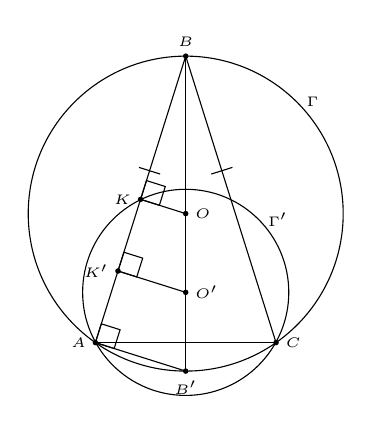
\begin{tikzpicture}[label distance=0mm]
  \coordinate (O) at (0, 0);
  \coordinate (A) at (-1.147, -1.638);
  \coordinate (B) at (0, 2);
  \coordinate (C) at (1.147, -1.638);
  \coordinate (B1) at (0, -2);
  \coordinate (K) at (-0.573, 0.181);
  \coordinate (O1) at (0, -1);
  \coordinate (K1) at (-0.860, -0.729);
  \coordinate (B1) at (0, -2);
  \draw (O) circle (2.0);
  \draw (O1) circle (1.309);
  \draw (A) -- (B);
  \draw (A) -- (C);
  \draw (B) -- (C);
  \draw (A) -- (B1);
  \draw (O) -- (K);
  \draw (O1) -- (K1);
  \draw (B) -- (B1);
  %%  \fill (O) circle[radius=1pt]  node [above, font=\tiny] {$O$};
  %% \fill (O1) circle[radius=1pt]  node [above, font=\tiny] {$O'$};
  \fill (K) circle[radius=1pt] node[left, font=\tiny] {$K$};
  \fill (K1) circle[radius=1pt] node[left, font=\tiny] {$K^\prime$};
  \fill (O) circle[radius=1pt]  node [right, font=\tiny] {$O$};
  \fill (O1) circle[radius=1pt]  node [right, font=\tiny] {$O^\prime$};
  \fill (B1) circle[radius=1pt]  node [below, font=\tiny] {$B^\prime$};
%  \Node[left, font=\tiny] at (K) {$K$};
%  \node[left, font=\tiny] at (K1) {$K'$};
  %% \node[right, font=\tiny] at (O) {$O$};
  %% \node[right, font=\tiny] at (O1) {$O^\prime$};
  \fill (A) circle[radius=1pt] node[left, font=\tiny] {$A$};
  \fill (B) circle[radius=1pt] node[above, font=\tiny] {$B$};
  \fill (C) circle[radius=1pt] node[right, font=\tiny] {$C$};
  \node[right, font=\tiny] at (1.414, 1.414) {$\Gamma$};
  \node[right, font=\tiny] at (0.925, -0.075) {$\Gamma'$};
  \tkzMarkSegment[pos=0.6, mark=|](A,B);
  \tkzMarkSegment[pos=0.6, mark=|](C,B);
  \tkzMarkRightAngle(B,A,B1);
  \tkzMarkRightAngle(B,K,O);
  \tkzMarkRightAngle(B,K1,O1);

\end{tikzpicture}
\end{document}
